\begin{frame}{Nonlinear problems}
  \begin{itemize}
  \item matrix-based smoothers require global linearization
  \item nonlinearity often more efficiently resolved locally
  \item nonlinear additive or multiplicative Schwarz
  \item nonlinear/matrix-free is good if
    \[ C = \frac{(\text{cost to evaluate residual at one point}) \cdot N}{(\text{cost of global residual})} \sim 1 \]
    \begin{itemize}
    \item finite difference: $C < 2$
    \item finite volume: $C \sim 2$, depends on reconstruction
    \item finite element: $C \sim \text{number of vertices per cell}$
    \end{itemize}
  \item larger block smoothers help reduce $C$
  \end{itemize}
  \vspace{-2.5em}
  \hfill 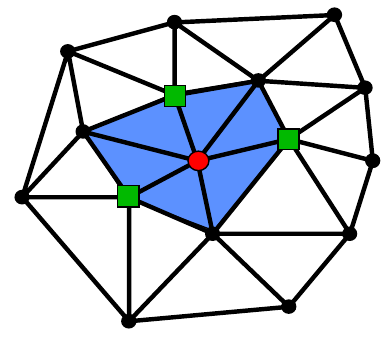
\includegraphics[width=0.3\textwidth]{figures/NodeStencil}
\end{frame}
